 \documentclass[11pt,a4paper]{article}
\usepackage[utf8]{inputenc}		% LaTeX, comprend les accents !
\usepackage[T1]{fontenc}
\usepackage{natbib}	
%\usepackage[square,sort&compress,sectionbib]{natbib}		% Doit être chargé avant babel      
\usepackage[frenchb,english]{babel}
\usepackage{lmodern}
\usepackage{amsmath,amssymb, amsthm}
\usepackage{a4wide}
\usepackage[capposition=top]{floatrow}
\usepackage{verbatim}
\usepackage{float}
\usepackage{placeins}
\usepackage{flafter}
\usepackage{longtable}
\usepackage{import}
\usepackage{pdflscape}
\usepackage{rotating}
\usepackage{hhline}
\usepackage{multirow}
\usepackage{booktabs}
\usepackage[pdftex,pdfborder={0 0 0},colorlinks=true,linkcolor=blue,urlcolor=blue,citecolor=blue,bookmarksopen=true]{hyperref}
\usepackage{eurosym}
%\usepackage{breakcites}
\usepackage[autostyle]{csquotes}
%\usepackage{datetime}
\usepackage{natbib}
\usepackage{setspace}
\usepackage{lscape}
\usepackage[usenames]{color}
\usepackage{indentfirst}
\usepackage{url}
\usepackage{enumitem}
\usepackage{multirow}
\usepackage{subcaption}
\usepackage[justification=centering]{caption}
\bibliographystyle{agsm}

\usepackage{array}

\newcommand{\isEmbedded}{true}

\graphicspath{{Figures/}}


\begin{document}

\selectlanguage{frenchb}
\title{Analyse des trajectoires dans les grilles \\ Focus sur les adjoints techniques}


\author{Simon Rabat\'e et Mahdi Ben Jelloul}


\maketitle

% Introduction
Ce note propose une première analyse des trajectoires indiciaires sur un sous-échantillon de la base carrière: les individus qui se trouvent dans le corps des adjoints techniques pour toutes les années entre 2007 et 2015. 

\renewcommand*\contentsname{\textsc{Plan de la note}}
\tableofcontents

\clearpage


% Section I: Analyse des grilles
\section{Le corps des adjoints techniques}

Le corps des adjoints techniques comporte quatre grades distincts: les adjoints technique de 2eme classe, les adjoints techniques de 1ere classe, les adjoints techniques principal de 2e classe et les adjoints technique principal de 1ere classe. 

Dans la suite de la note nous utilisons les abréviations suivantes pour ces différents grades: AT2, AT1, ATP2 et ATP1 respectivement. 

Le tableau ci-dessous précise les conditions de passage au grade immédiatement supérieur\footnote{Source: \url{http://www.cdg45.fr/racine/accueil/gestion_des_ressources_humaines/cadres_d_emplois_de_la_fpt/filiere_technique/adjoint_technique_territorial/avancement_de_grade/avancement_de_grade}.}. 



\begin{table}[h!]
\label{means}
\centering
\caption{Conditions d'avancement pour le corps des AT} 
\begin{tabular}{l|c|ccc}
\toprule
 Grade  & Type d'avancement&  \multicolumn{3}{c}{||| Condition de .. |||}  \\
		&  				   &  Durée dans le grade	&  Échelon	dans le grade & Durée dans l'échelon \\
\midrule
AT2  &	Avec exam pro. 	&   3 ans  & 	4  & NA \\
AT2  &	Sans exam pro. 	& 	10 ans &	7  &	NA \\
AT1  & Tous				& 	6 ans  &	5  &	NA \\
ATP2 & Tous				& 	5 ans  &	6  &	2 ans  \\	
%	
\bottomrule
\end{tabular}
\end{table}

Les grilles de ces différents grades ont connu de nombreuses évolutions dans les années considérées (4 pour les trois premiers, 6 pour le grade ATP1). Les graphiques \ref{echelon_by_neg} et \ref{echelon_by_date} proposent une visualisation de ces différentes grilles. 



\begin{figure}[ht] 
  \caption{Evolution des grilles: grade par grade}
  \label{echelon_by_neg} 
  \begin{subfigure}[b]{0.55\linewidth}
      \caption{Grade AT2} 
    \label{echelon_by_neg_0} 
    \centering
    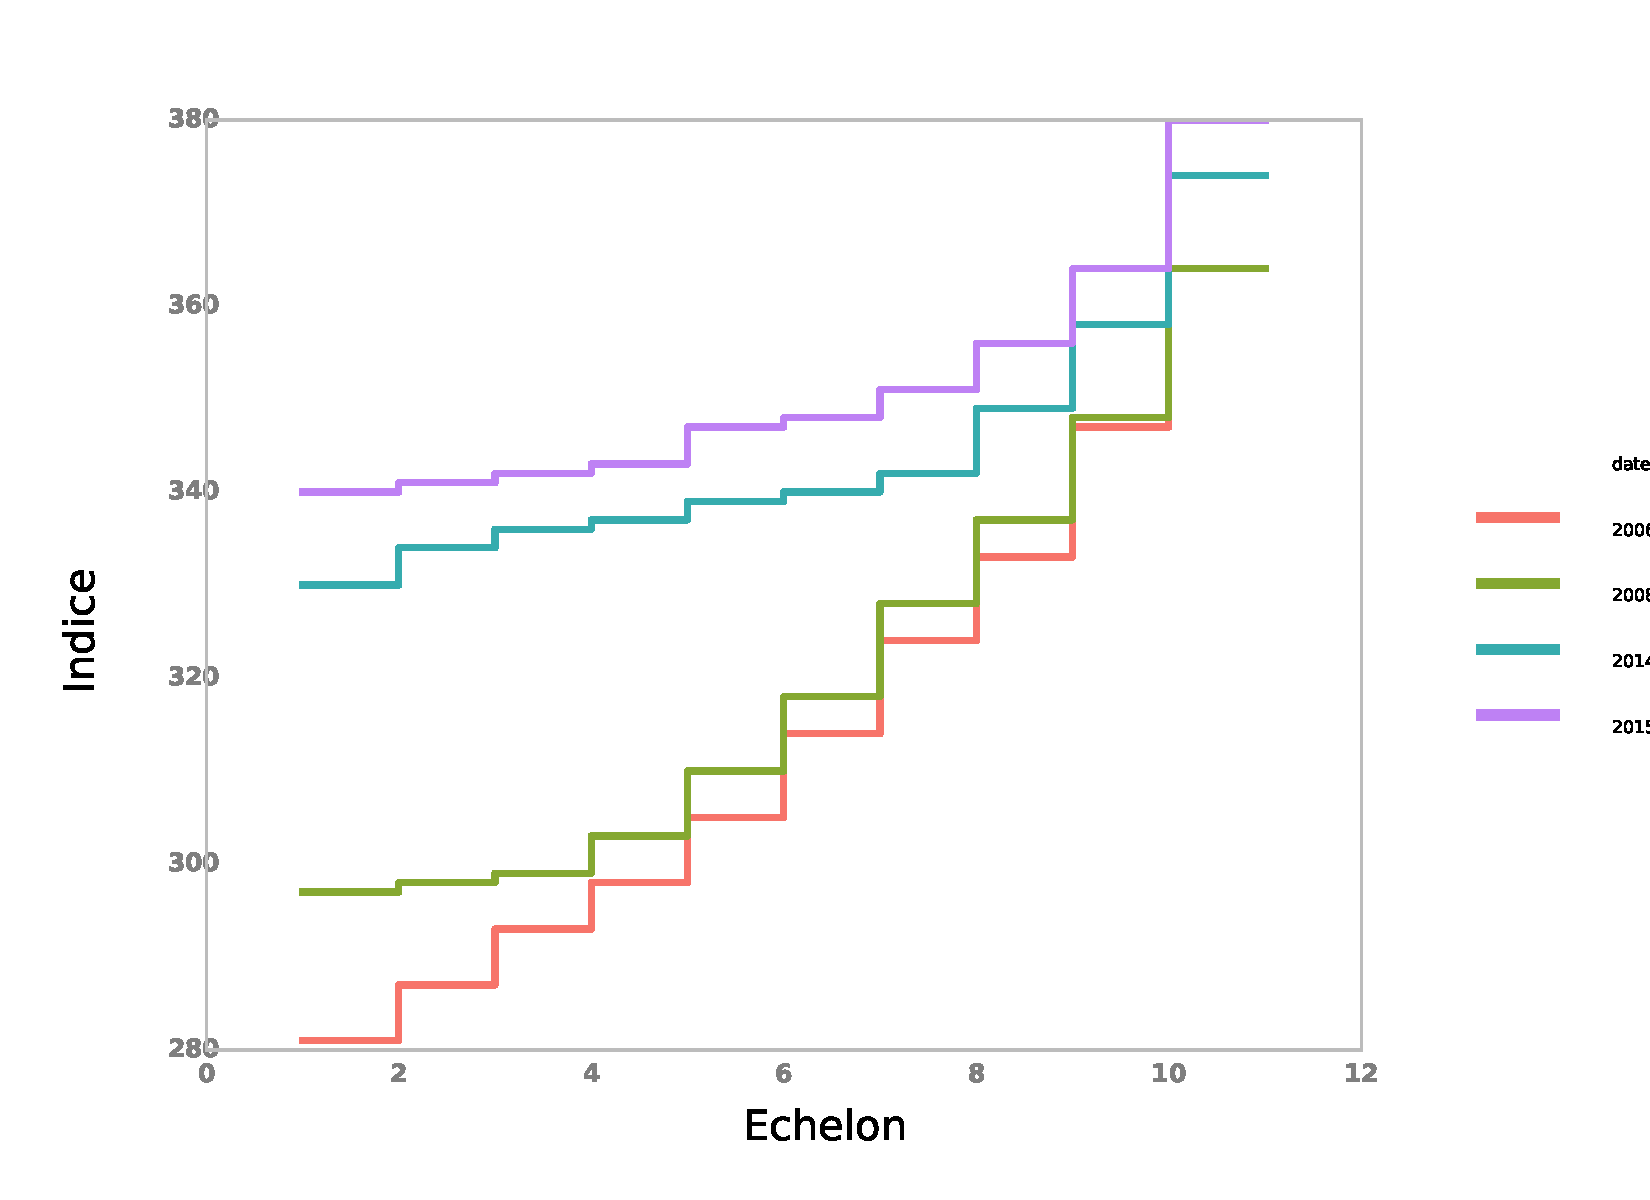
\includegraphics[width=1\linewidth]{0_grille_by_neg.pdf} 
    \vspace{4ex}
  \end{subfigure}%% 
  \begin{subfigure}[b]{0.55\linewidth}
        \caption{Grade AT1} 
    \label{echelon_by_neg_1} 
    \centering
    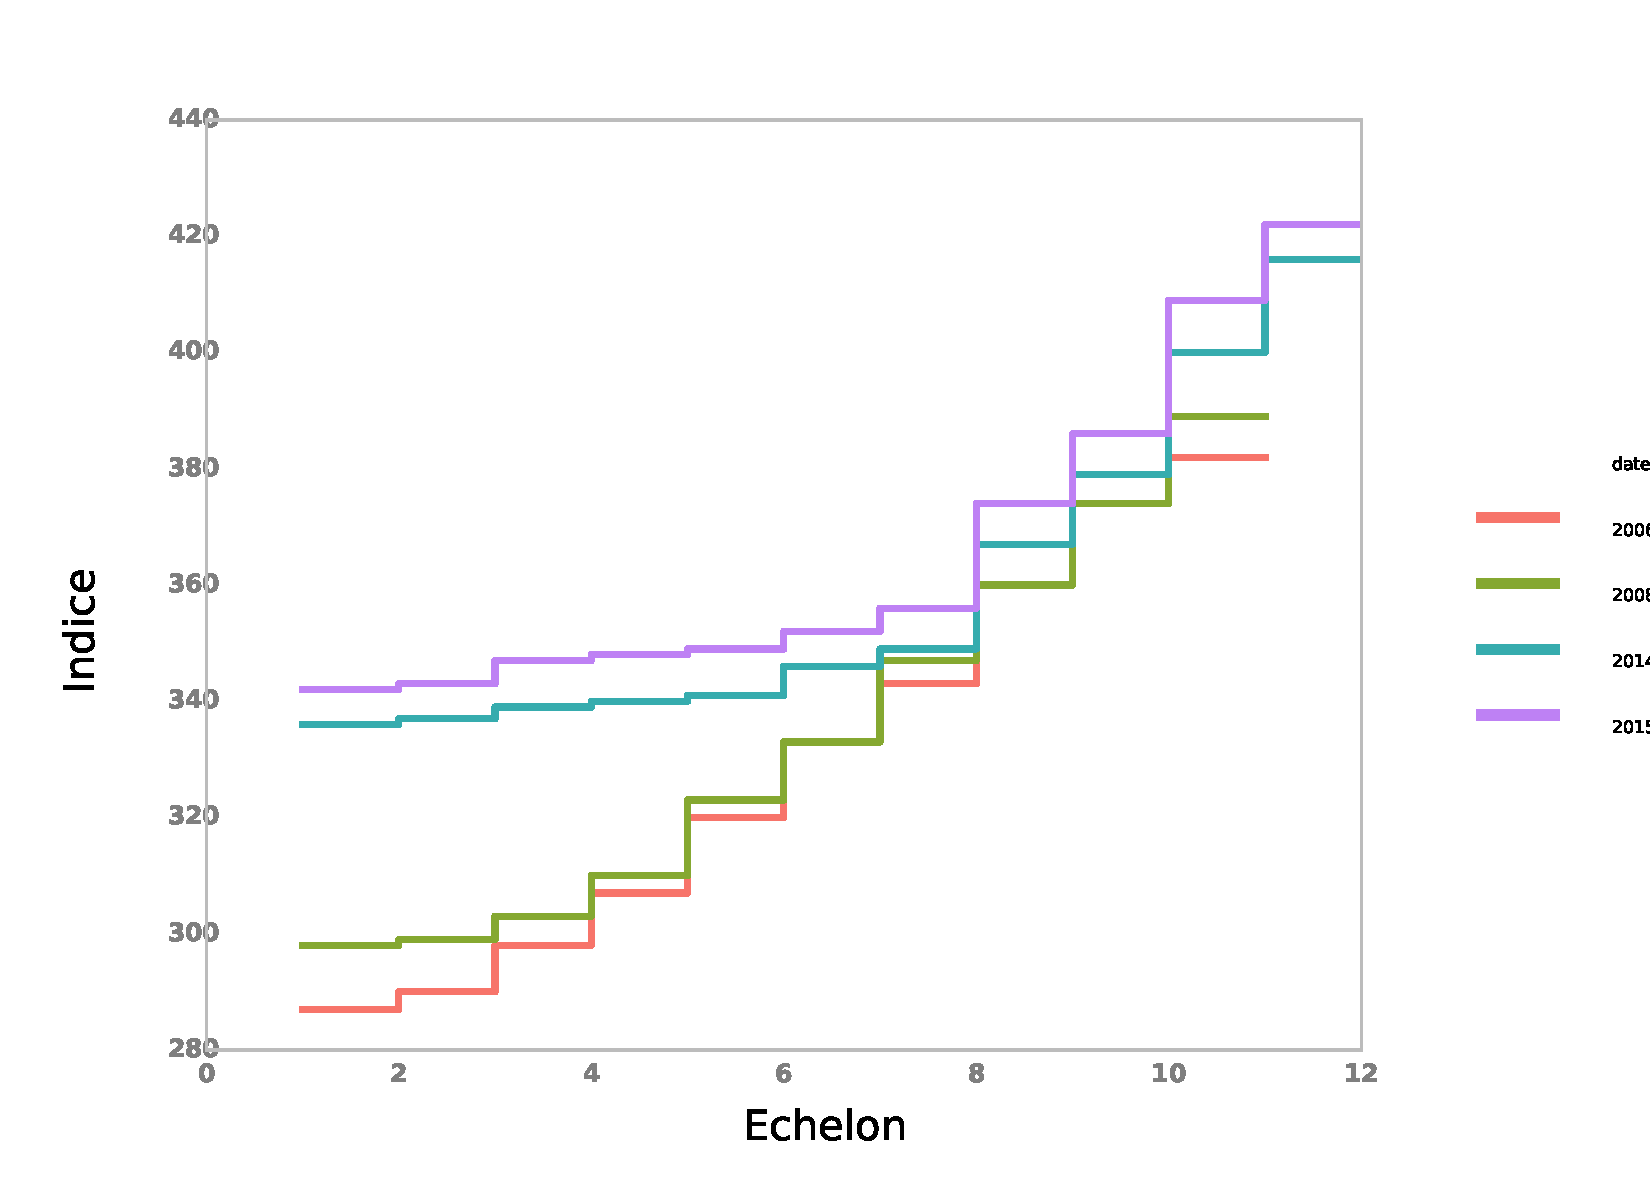
\includegraphics[width=1\linewidth]{1_grille_by_neg.pdf} 
    \vspace{4ex}
  \end{subfigure} 
  \begin{subfigure}[b]{0.55\linewidth}
        \caption{Grade ATP2} 
    \label{echelon_by_neg_2} 
    \centering
    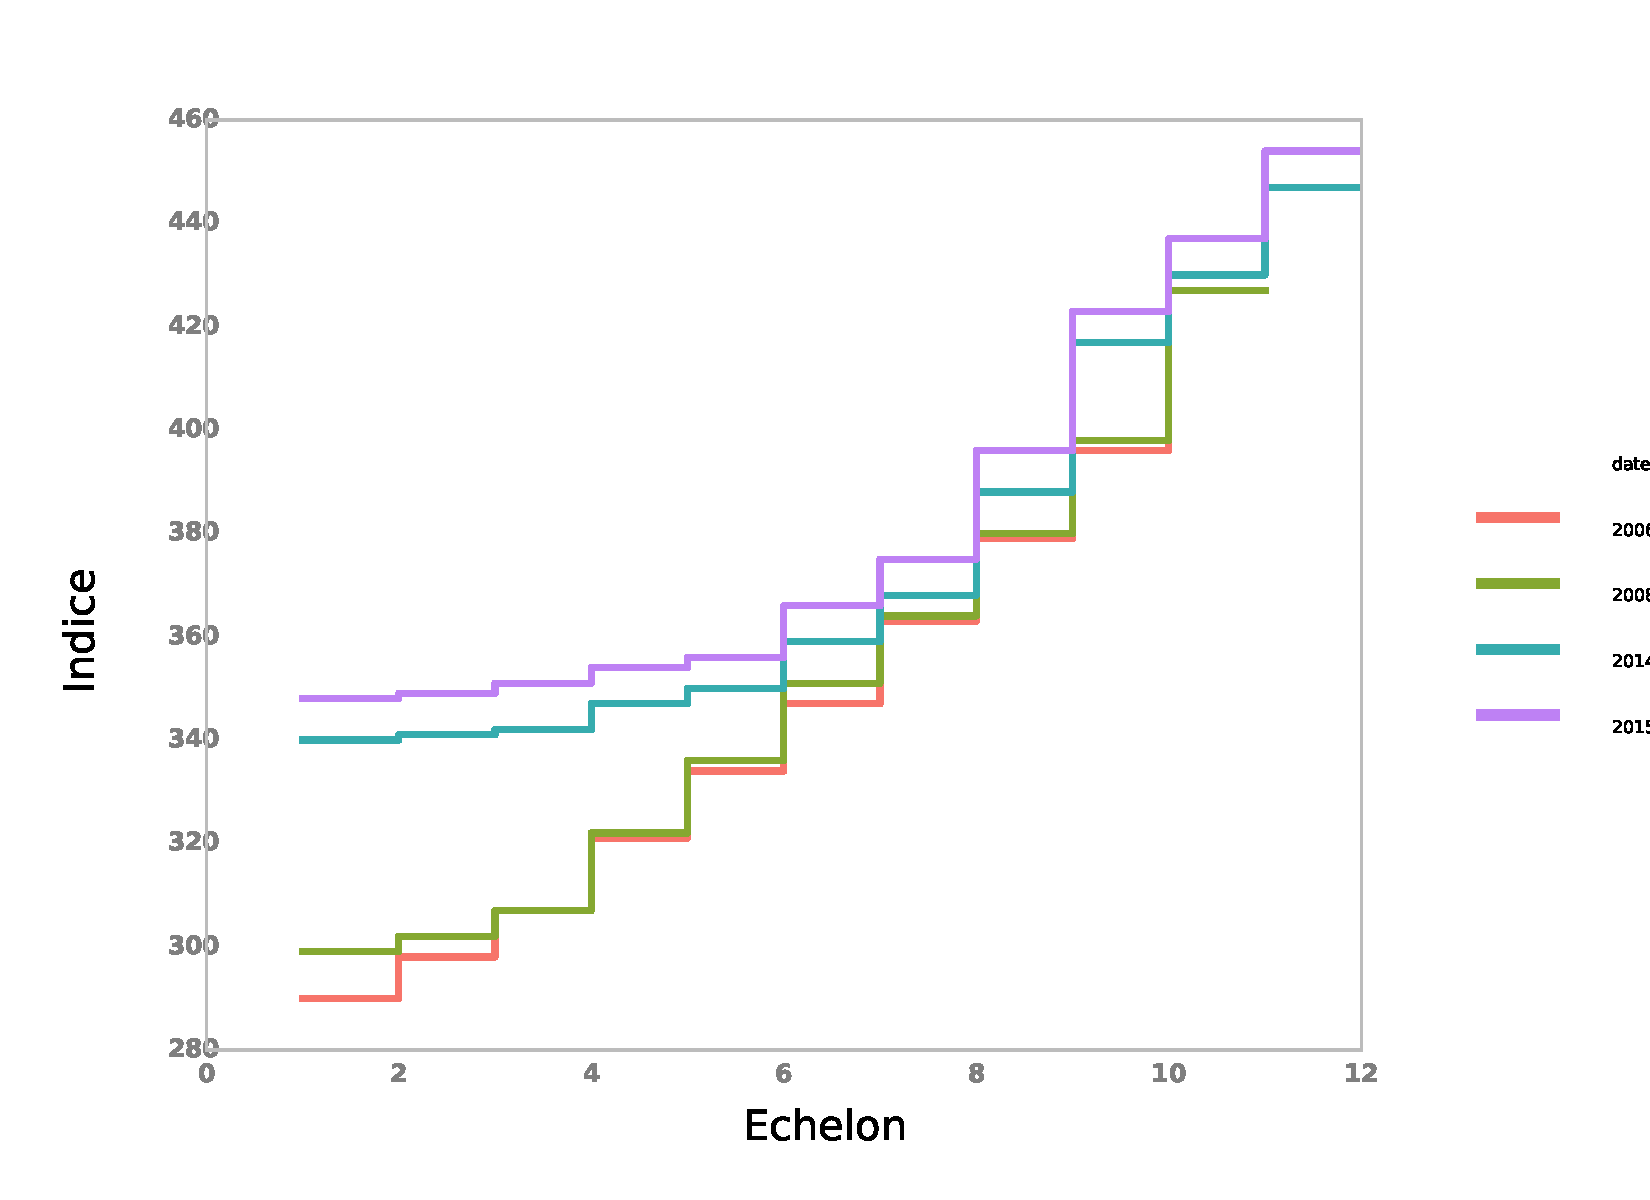
\includegraphics[width=1\linewidth]{2_grille_by_neg.pdf} 
  \end{subfigure}%%
  \begin{subfigure}[b]{0.55\linewidth}
        \caption{Grade ATP1} 
    \label{echelon_by_neg_3} 
    \centering
    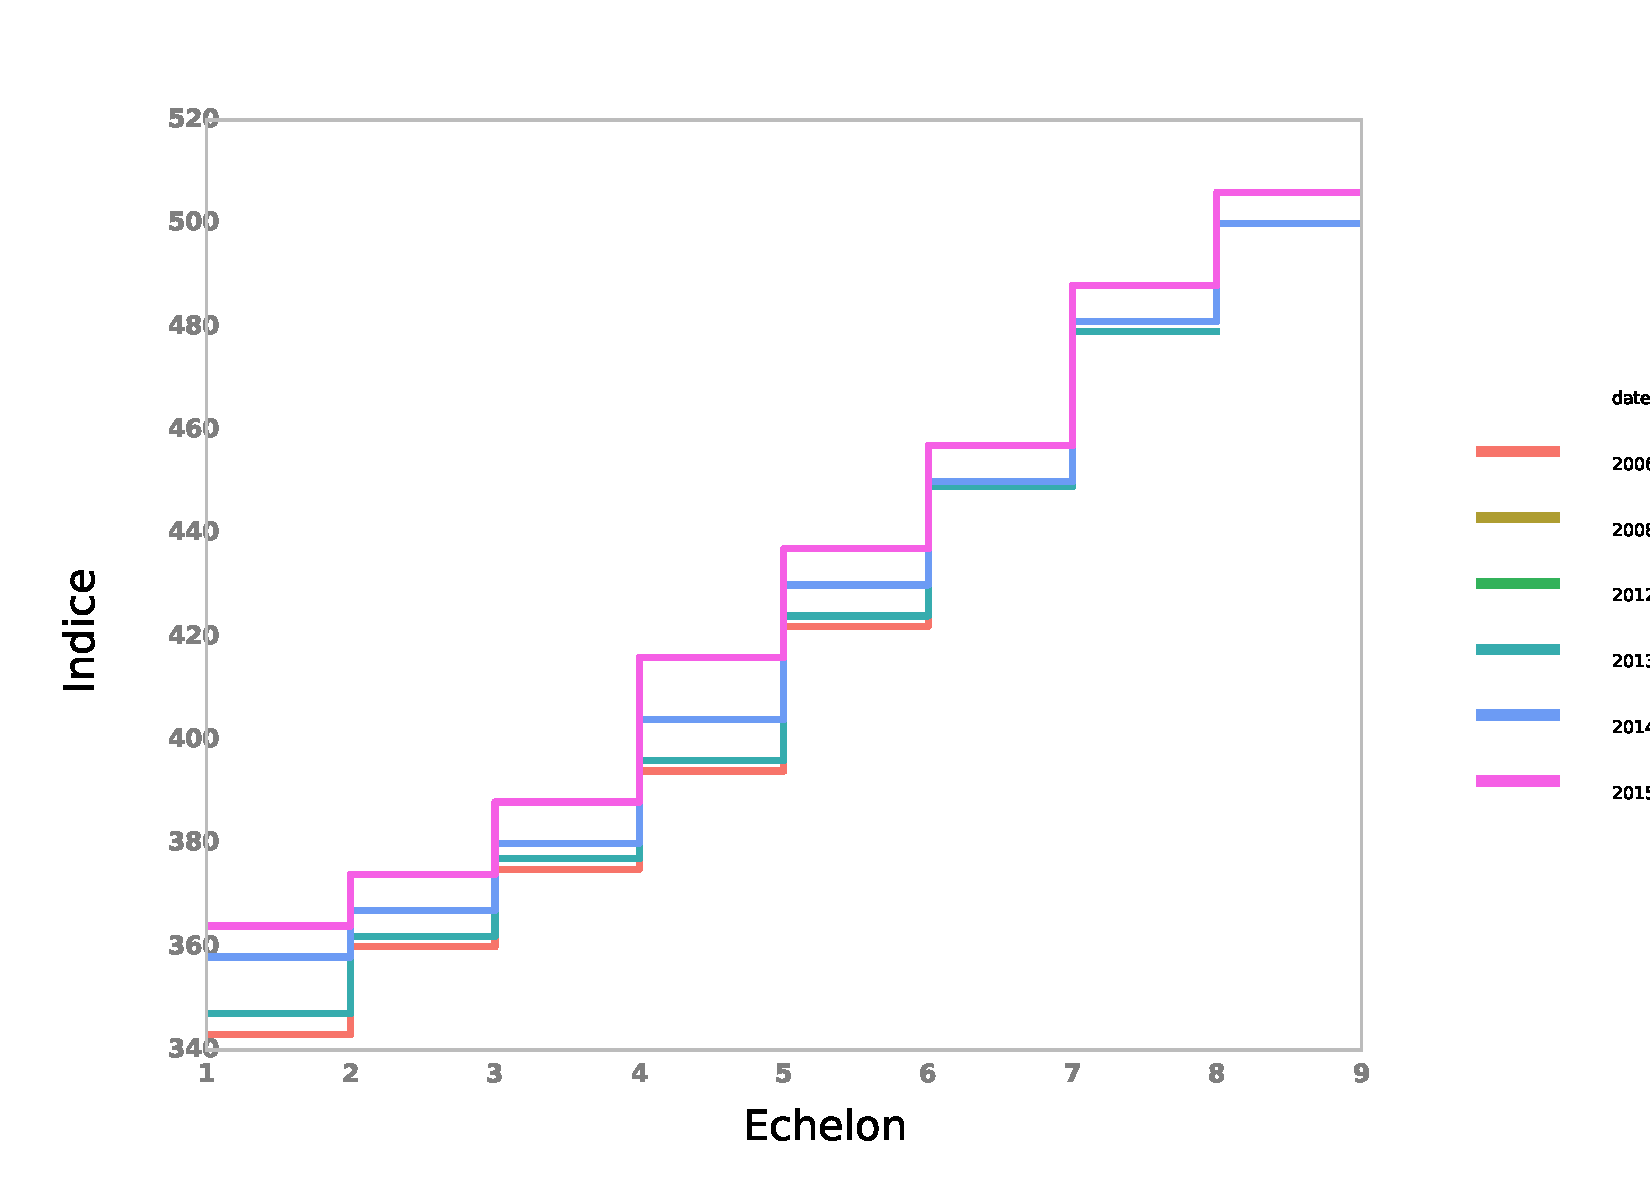
\includegraphics[width=1\linewidth]{3_grille_by_neg.pdf} 
  \end{subfigure} 
\end{figure}




\begin{figure}[ht] 
  \caption{Évolution des grilles: niveau relatif des grades}
  \label{echelon_by_date} 
  \begin{subfigure}[b]{0.55\linewidth}
      \caption{Année 2006} 
    \label{echelon_by_neg_0} 
    \centering
    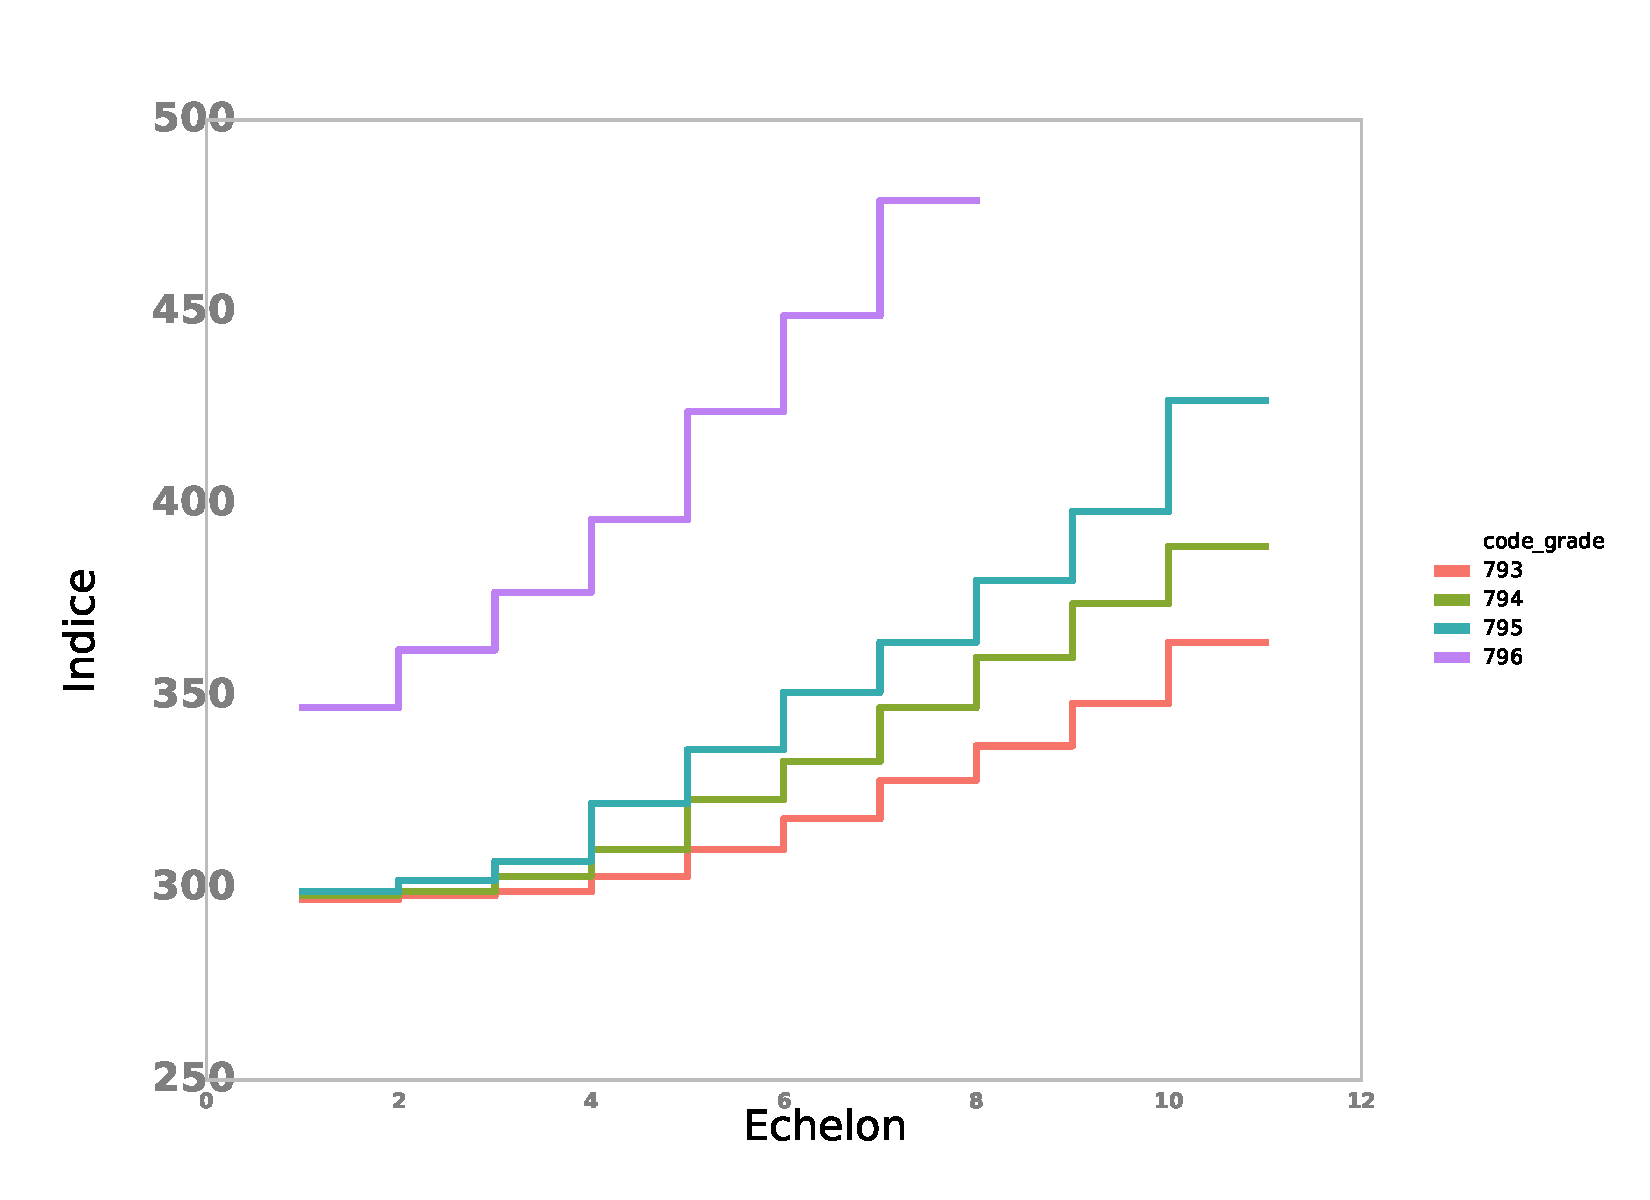
\includegraphics[width=1\linewidth]{0_grille_by_date.pdf} 
    \vspace{4ex}
  \end{subfigure}%% 
  \begin{subfigure}[b]{0.55\linewidth}
      \caption{Année 2008} 
    \label{echelon_by_neg_1} 
    \centering
    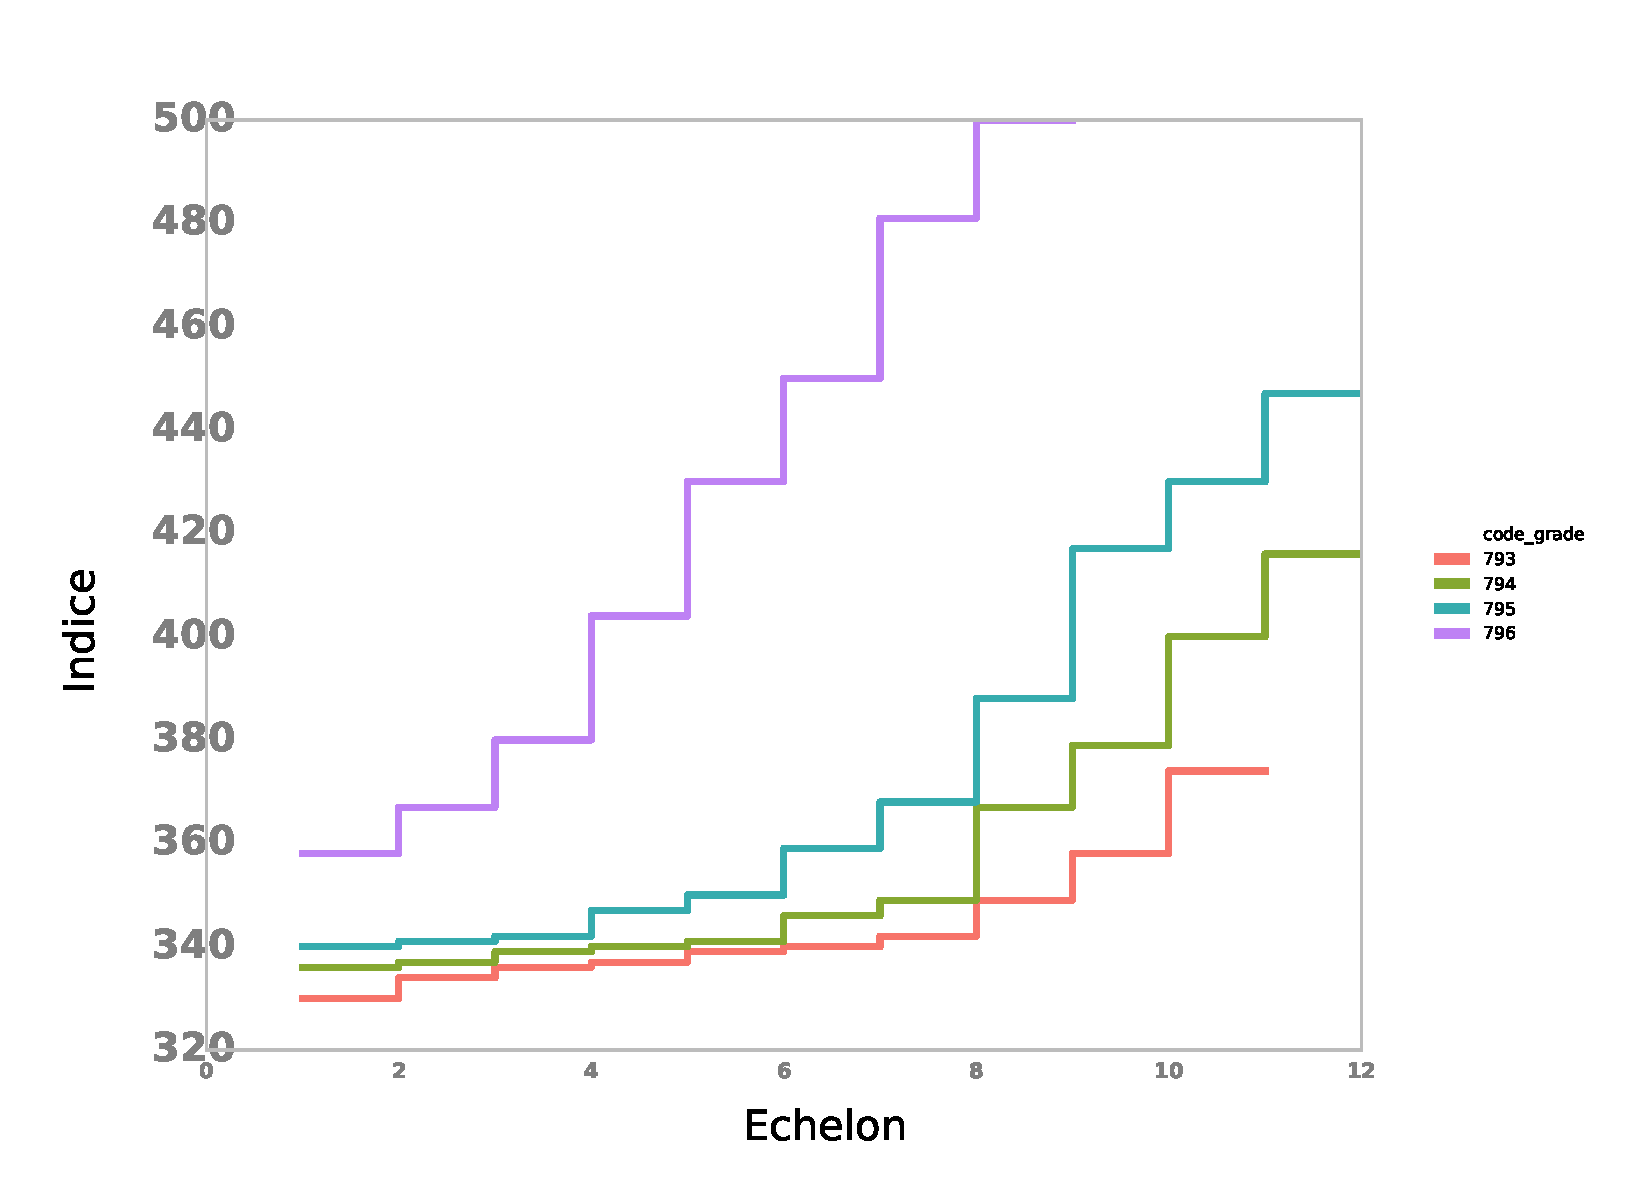
\includegraphics[width=1\linewidth]{1_grille_by_date.pdf} 
    \vspace{4ex}
  \end{subfigure} 
  \begin{subfigure}[b]{0.55\linewidth}
      \caption{Année 2014} 
    \label{echelon_by_neg_2} 
    \centering
    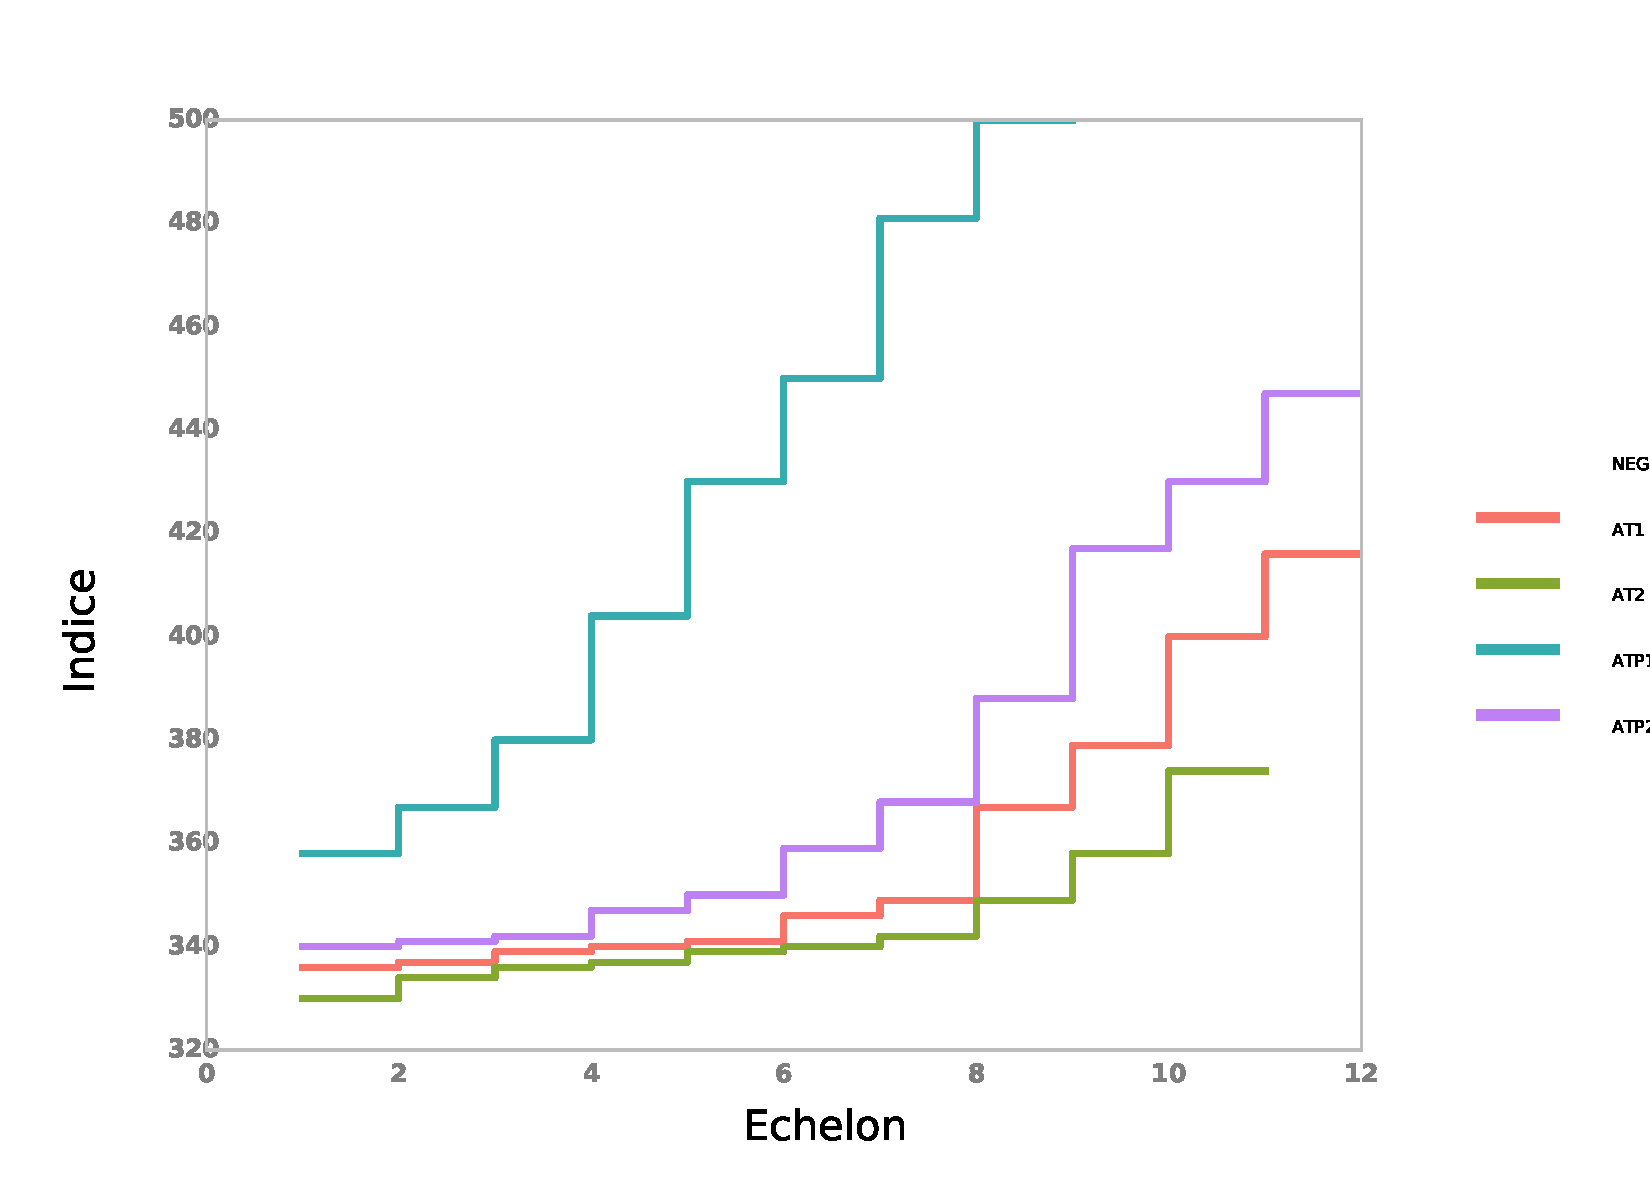
\includegraphics[width=1\linewidth]{2_grille_by_date.pdf} 
  \end{subfigure}%%
  \begin{subfigure}[b]{0.55\linewidth}
      \caption{Année 2015} 
    \label{echelon_by_neg_3} 
    \centering
    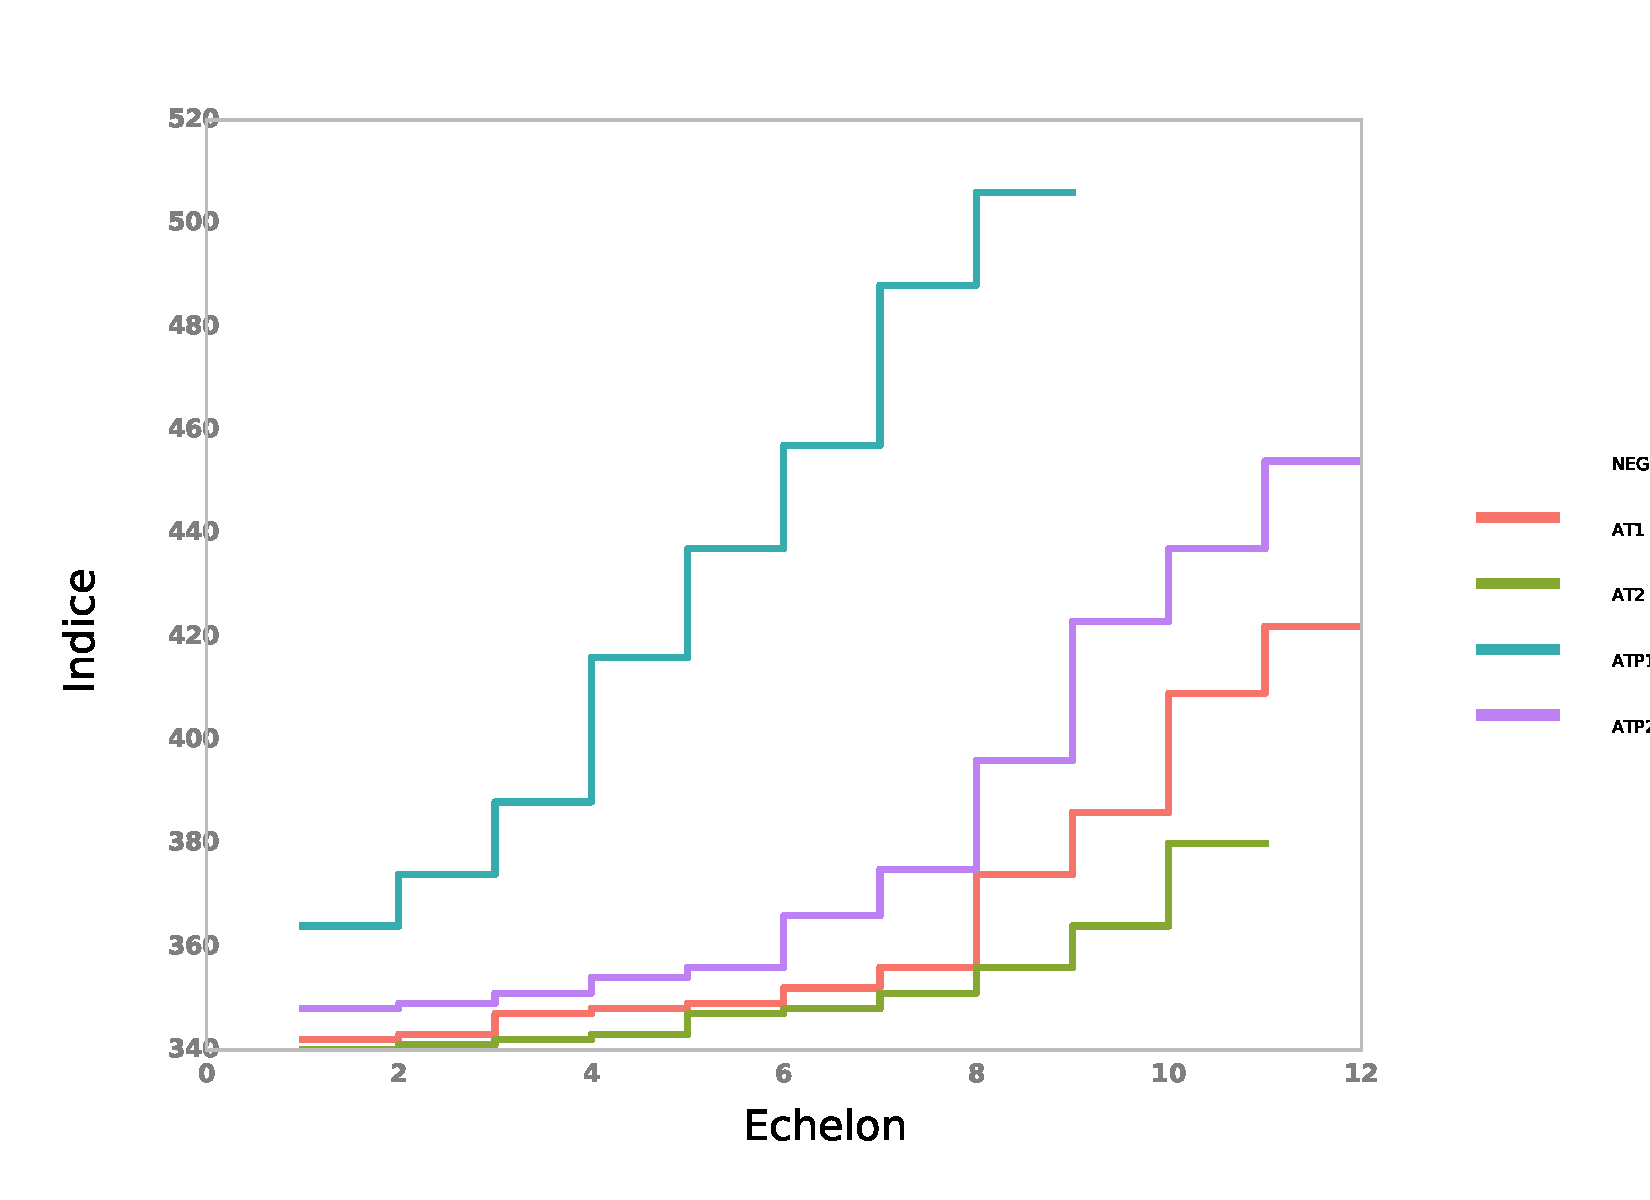
\includegraphics[width=1\linewidth]{3_grille_by_date.pdf} 
  \end{subfigure} 
\end{figure}




\clearpage





% Section II: Travail sur les données
\section{Point sur les données}


\subsection{Sélection de l'échantillon}

Nous nous concentrons sur les individus, nés entre 1960 et 1999, et ayant passé au moins une année dans l'un des grades du corps. Nous supprimons les individus apparaissant deux fois (environ 250). Nous obtenus un échantillon initial de 546709 individus. 

L'étude des transitions entre grades et échelon nécessite de pouvoir identifier clairement les moments où le grade et l'échelon changent. La difficulté est alors la suivante: une information manquante pour l'une des variables clés rend difficile l'analyse de la séquence globale pour l'individu, car nous ne pouvons différencier une information manquante d'un changement dans la carrière. Le choix est pour l'instant fait de se concentrer sur une population très restrictive, en ne gardant que les individus pour lesquels nous pouvons reconstituer la carrière de manière précise. L'objectif est de se concentrer sur l'aspect modélisation de la question à ce stade. 

Nous appliquons donc les filtres suivants à la base initiale. L'impact sur la taille de l'échantillon de ces filtres successifs est présenté à la table \ref{filters}. La règle appliquée est la suivante: dès que les conditions sont remplies pour au moins une observation, nous retirons l'ensemble des observations pour l'individus en question. 
\begin{enumerate}[leftmargin=1cm ,parsep=0cm,itemsep=0cm,topsep=0cm] 
\item[F1] Garder uniquement les individus pour lesquels le libemploi n'est pas manquant quand l'indice ou le statut ne sont pas nuls. Nous perdons alors 15\% des individus, ce qui est relativement important par rapport à ce qui était attendu. 
\item[F2] Garder uniquement individus pour lesquels tous les grades sont renseignés, quand la variable libemploi n'est pas nulle. Cela implique de supprimer tous les individus pour lesquels les procédures d'imputation des libellés n'ont pas permis d'attribuer un grade neg pour chaque libemploi. Nous perdons ainsi 35\% des individus, ce qui était attendu. 
\item[F3] Garder uniquement les individus pour lesquels l'échelon est renseigné pour les années dans le corps. Ce filtre a un effet fort et inattendu, puisque l'on perd encore presque 40\% des individus. Par ailleurs cet effet est très hétérogène en fonction des grades. A cette étape les échelons manquant représentent environ 15\% des observations pour le grade AT2, contre 90\% pour le grade ATP2.
\end{enumerate}



\begin{table}[h!]
\centering
\caption{Impact des filtres successifs sur la taille de l'échantillon} 
\label{filters}
\begin{tabular}{lcc}
\toprule
 & Nb d'individus & \% echantillon initial \\ 
  \hline
Echantillon initial & 10000 & 100 \\ 
F1: Libemploi manquant quand statut non vide & 8595 & 86 \\ 
  F2: Neg manquant quand libemploi renseigné & 4881 & 49 \\ 
  F3: Echelon manquant quand neg dans AT & 1193 & 12 \\ 
\bottomrule
\end{tabular}
\end{table}


Estimer les modèles sur une si faible part de la population d'intérêt est susceptible de poser des problèmes, peut-être en termes de nombre d'observations mais surtout en termes de validité externe. Plus la population d'estimation est spécifique, moins la modélisation des comportements est susceptible d'être généralisable à l'ensemble de la population. 


Questions et pistes amélioration pour augmenter la taille de l'échantillon retenu pour l'analyse: 
\begin{itemize}[leftmargin=1cm ,parsep=0cm,itemsep=0cm,topsep=0cm] 
\item Améliorer le remplissage des neg 
	\begin{enumerate}[leftmargin=1cm ,parsep=0cm,itemsep=0cm,topsep=0cm] 
	\item Poursuivre le matching
	\item Renseigner des grades à la main 
	\item Matching sur une sous-population de libellés des individus ayant au moins un NEG dans le corps
	\end{enumerate}
\item Correction du grade à partir de l'indice. 
\item Échelon = - 1?
\item Utilisation de l'information infra
\end{itemize}


\subsection{Sélection de l'échantillon}


\subsection{Censure des données}

Par exemple, si l'on prend la grille qui a cours en 2008, la durée minimale (resp. maximale) pour parcourir l'ensemble du grade est de 21 (resp. 30) ans. Si la plupart des individus ne parcoure pas l'ensemble d'un grade, 

NB: pas censure totale, possibilité d'utiliser les informations sur les libellés avant 2007, et sur les variables individuelles: date d'affiliation etc. 





% Section III: Statistiques descriptives
\section{Analyse des trajectoires}

\subsection{Statistiques descriptives}


\subsection{Survie dans le grade}





\section{Résumé et liste des points à aborder en priorité}


\begin{itemize}
\item Amélioration des données 
\begin{enumerate}
\item Poursuivre matching
\item Améliorer l'attribution de l'échelon
\item Pourquoi tant d'hétérogénéité par échelon? 
\end{enumerate}
\end{itemize}


\end{document}


